\documentclass[12pt]{report}
\usepackage[utf8]{inputenc}
\usepackage[russian]{babel}
%\usepackage[14pt]{extsizes}
\usepackage{listings}
\usepackage{graphicx}
\usepackage{amsmath,amsfonts,amssymb,amsthm,mathtools} 
\usepackage{pgfplots}
\usepackage{filecontents}
\usepackage{indentfirst}
\usepackage{eucal}
\usepackage{amsmath}
\usepackage{enumitem}
\frenchspacing

\usepackage{indentfirst} % Красная строка


\usetikzlibrary{datavisualization}
\usetikzlibrary{datavisualization.formats.functions}

\usepackage{amsmath}




% Для листинга кода:
\lstset{ %
language=haskell,                 % выбор языка для подсветки (здесь это С)
basicstyle=\small\sffamily, % размер и начертание шрифта для подсветки кода
numbers=left,               % где поставить нумерацию строк (слева\справа)
numberstyle=\tiny,           % размер шрифта для номеров строк
stepnumber=1,                   % размер шага между двумя номерами строк
numbersep=5pt,                % как далеко отстоят номера строк от подсвечиваемого кода
showspaces=false,            % показывать или нет пробелы специальными отступами
showstringspaces=false,      % показывать или нет пробелы в строках
showtabs=false,             % показывать или нет табуляцию в строках
frame=single,              % рисовать рамку вокруг кода
tabsize=2,                 % размер табуляции по умолчанию равен 2 пробелам
captionpos=t,              % позиция заголовка вверху [t] или внизу [b] 
breaklines=true,           % автоматически переносить строки (да\нет)
breakatwhitespace=false, % переносить строки только если есть пробел
escapeinside={\#*}{*)}   % если нужно добавить комментарии в коде
}

\usepackage[left=2cm,right=2cm, top=2cm,bottom=2cm,bindingoffset=0cm]{geometry}
% Для измененных титулов глав:
\usepackage{titlesec, blindtext, color} % подключаем нужные пакеты
\definecolor{gray75}{gray}{0.75} % определяем цвет
\newcommand{\hsp}{\hspace{20pt}} % длина линии в 20pt
% titleformat определяет стиль
\titleformat{\chapter}[hang]{\Huge\bfseries}{\thechapter\hsp\textcolor{gray75}{|}\hsp}{0pt}{\Huge\bfseries}


% plot
\usepackage{pgfplots}
\usepackage{filecontents}
\usetikzlibrary{datavisualization}
\usetikzlibrary{datavisualization.formats.functions}

\begin{document}
%\def\chaptername{} % убирает "Глава"
\thispagestyle{empty}
\begin{titlepage}
	\noindent \begin{minipage}{0.15\textwidth}
	
\includegraphics[width=\linewidth]{b_logo}
	\end{minipage}
	\noindent\begin{minipage}{0.9\textwidth}\centering
		\textbf{Министерство науки и высшего образования Российской Федерации}\\
		\textbf{Федеральное государственное бюджетное образовательное учреждение высшего образования}\\
		\textbf{~~~«Московский государственный технический университет имени Н.Э.~Баумана}\\
		\textbf{(национальный исследовательский университет)»}\\
		\textbf{(МГТУ им. Н.Э.~Баумана)}
	\end{minipage}
	
	\noindent\rule{18cm}{3pt}
	\newline\newline
	\noindent ФАКУЛЬТЕТ $\underline{\text{«Информатика и системы управления»}}$ \newline\newline
	\noindent КАФЕДРА $\underline{\text{«Программное обеспечение ЭВМ и информационные технологии»}}$\newline\newline\newline\newline\newline
	
	
	\begin{center}
		\noindent\begin{minipage}{1.3\textwidth}\centering
			\Large\textbf{  Отчёт по лабораторной работе №2}\newline
			\textbf{по дисциплине "Анализ алгоритмов"}\newline\newline
		\end{minipage}
	\end{center}
	
	\noindent\textbf{Тема} $\underline{\text{Умножение матриц}}$\newline\newline
	\noindent\textbf{Студент} $\underline{\text{Романов А.В.}}$\newline\newline
	\noindent\textbf{Группа} $\underline{\text{ИУ7-53Б}}$\newline\newline
	\noindent\textbf{Оценка (баллы)} $\underline{\text{~~~~~~~~~~~~~~~~~~~~~~~~~~~}}$\newline\newline
	\noindent\textbf{Преподаватели} $\underline{\text{Волкова Л.Л., Строганов Ю.В.}}$\newline\newline\newline
	
	\begin{center}
		\vfill
		Москва~---~\the\year
		~г.
	\end{center}
\end{titlepage}


\tableofcontents

\newpage
\chapter*{Введение}
\addcontentsline{toc}{chapter}{Введение}
Алгоритм Копперсмита — Винограда — алгоритм умножения квадратных матриц, предложенный в 1987 году Д. Копперсмитом и Ш. Виноградом.
В исходной версии асимптотическая сложность алгоритма составляла $O(n^{2,3755})$, где  $n$ — размер стороны матрицы.

Алгоритм Копперсмита — Винограда, с учётом серии улучшений и доработок в последующие годы, обладает лучшей асимптотикой среди известных алгоритмов умножения матриц.

На практике алгоритм Копперсмита — Винограда не используется, так как он имеет очень большую константу пропорциональности и начинает выигрывать в быстродействии у других известных алгоритмов только для матриц, размер которых превышает память современных компьютеров.
Поэтому пользуются алгоритмом Штрассена по причинам простоты реализации и меньшей константе в оценке трудоемкости.

Задачи лабораторной работы:

\begin{enumerate}

	\item Изучение и реализация трёх алгоритмов умножения матриц: обычный, Копперсмита-Винограда, оптимизированный Копперсмита-Винограда;
	\item Сравнительный анализ трудоёмкости алгоритмов на основе теоретических расчетов и выбранной модели вычислений;
	\item Сравнительный анализ алгоритмов на основе экспериментальных данных;

\end{enumerate}

\chapter{Аналитическая часть}


\section{Стандартный алгоритм}

Пусть даны две прямоугольные матрицы
\begin{equation}
	A_{lm} = \begin{pmatrix}
		a_{11} & a_{12} & \ldots & a_{1m}\\
		a_{21} & a_{22} & \ldots & a_{2m}\\
		\vdots & \vdots & \ddots & \vdots\\
		a_{l1} & a_{l2} & \ldots & a_{lm}
	\end{pmatrix},
	\quad
		B_{mn} = \begin{pmatrix}
		b_{11} & b_{12} & \ldots & b_{1n}\\
		b_{21} & b_{22} & \ldots & b_{2n}\\
		\vdots & \vdots & \ddots & \vdots\\
		b_{m1} & b_{m2} & \ldots & b_{mn}
	\end{pmatrix},
\end{equation}

тогда матрица $C$
\begin{equation}
	C_{ln} = \begin{pmatrix}
		c_{11} & c_{12} & \ldots & c_{1n}\\
		c_{21} & c_{22} & \ldots & c_{2n}\\
		\vdots & \vdots & \ddots & \vdots\\
		c_{l1} & c_{l2} & \ldots & c_{ln}
	\end{pmatrix},
\end{equation}

где
\begin{equation}
	\label{eq:M}
	c_{ij} =
		\sum_{r=1}^{m} a_{ir}b_{rj} \quad (i=\overline{1,l}; j=\overline{1,n})
\end{equation}

будет называться произведением матриц $A$ и $B$.
Стандартный алгоритм реализует данную формулу.

\section{Алгоритм Копперсмита -- Винограда}

Если посмотреть на результат умножения двух матриц, то видно, что каждый элемент в нем представляет собой скалярное произведение соответствующих строки и столбца исходных матриц.
Можно заметить также, что такое умножение допускает предварительную обработку, позволяющую часть работы выполнить заранее.

Рассмотрим два вектора $V = (v_1, v_2, v_3, v_4)$ и $W = (w_1, w_2, w_3, w_4)$.
Их скалярное произведение равно: $V \cdot W = v_1w_1 + v_2w_2 + v_3w_3 + v_4w_4$, что эквивалентно (\ref{for:new}):
\begin{equation}
	\label{for:new}
		V \cdot W = (v_1 + w_2)(v_2 + w_1) + (v_3 + w_4)(v_4 + w_3) - v_1v_2 - v_3v_4 - w_1w_2 - w_3w_4.
\end{equation}

Несмотря на то, что второе выражение требует вычисления большего количества операций, чем стандартный алгоритм: вместо четырёх умножений - шесть, а вместо трёх сложений - десять, выражение в правой части последнего равенства допускает предварительную обработку: его части можно вычислить заранее и запомнить для каждой строки первой матрицы и для каждого столбца второй, что позволит для каждого элемента выполнять лишь два умножения и пять сложений, складывая затем только лишь с 2 предварительно посчитанными суммами соседних элементов текущих строк и столбцов.
Из-за того, что операция сложения быстрее операции умножения в ЭВМ, на практике алгоритм должен работать быстрее стандартного.

\section{Вывод}
	В данном разделе были рассмотрены алгоритмы классического умножения матриц и алгоритм Винограда, основное отличие которого от классического алгоритма — наличие предварительной обработки, а также количество операций умножения. 
\clearpage

\chapter{Конструкторская часть}

\section{Схемы алгоритмов}

На рисунке \ref{img:simple} приведена схема стандартного алгоритма умножения матриц.


На рисунках \ref{img:vino} и \ref{img:mv_mh} представлена схема алгоритма Копперсмита — Винограда.

На рисунках \ref{img:vino_improved} и \ref{img:mv_mh_fast} представлена схема оптимизированного алгоритма Копперсмита — Винограда.

\begin{figure}[h]
	\centering
	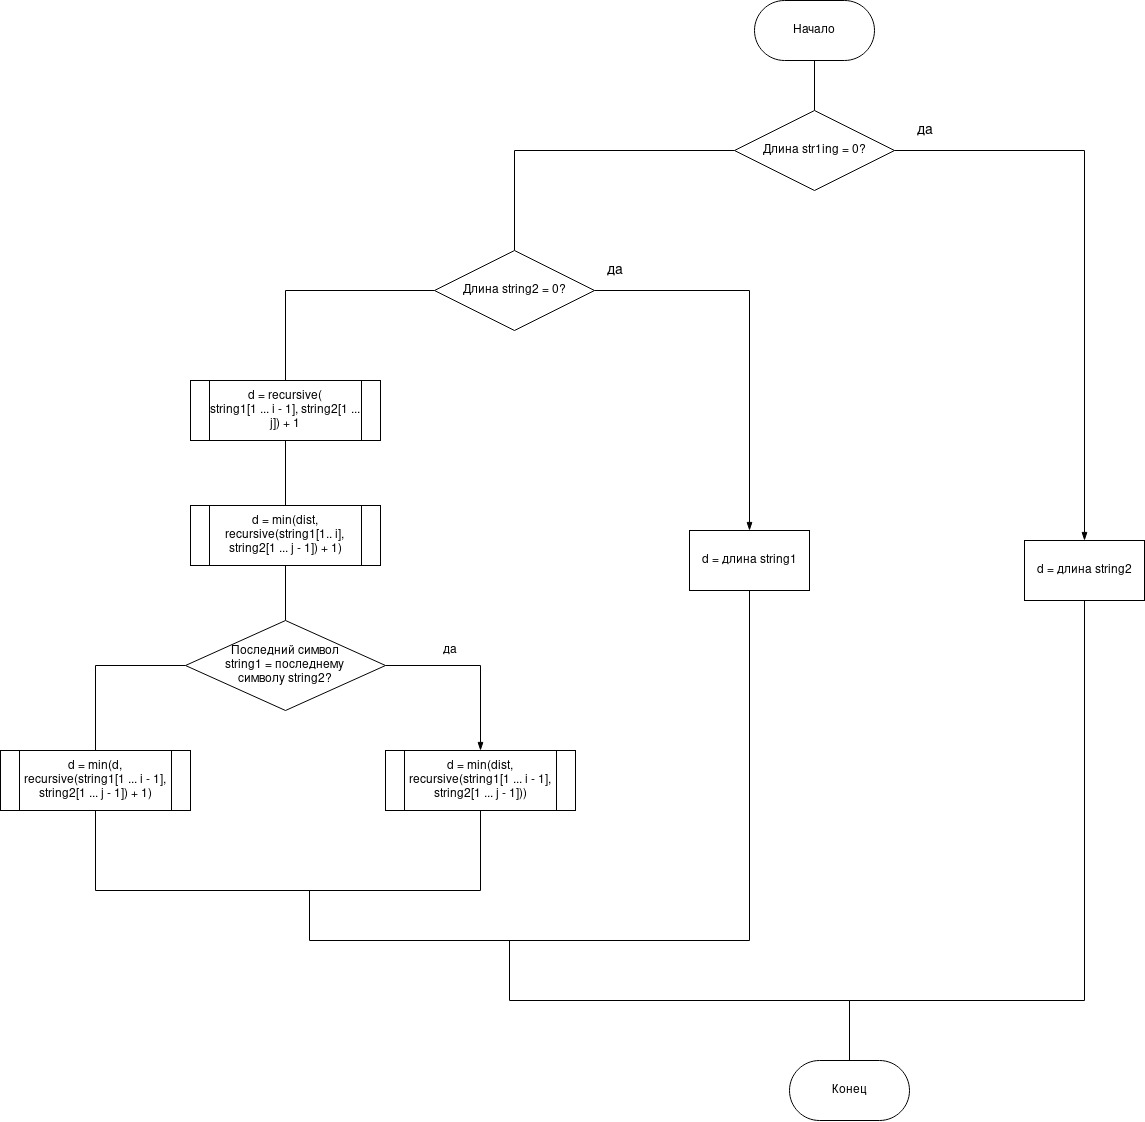
\includegraphics[width=0.75\linewidth]{rec.jpg}
	\caption{Схема рекурсивного алгоритма нахождения расстояния Левенштейна}
	\label{fig:mpr}
\end{figure}

\begin{figure}[h]
	\centering
	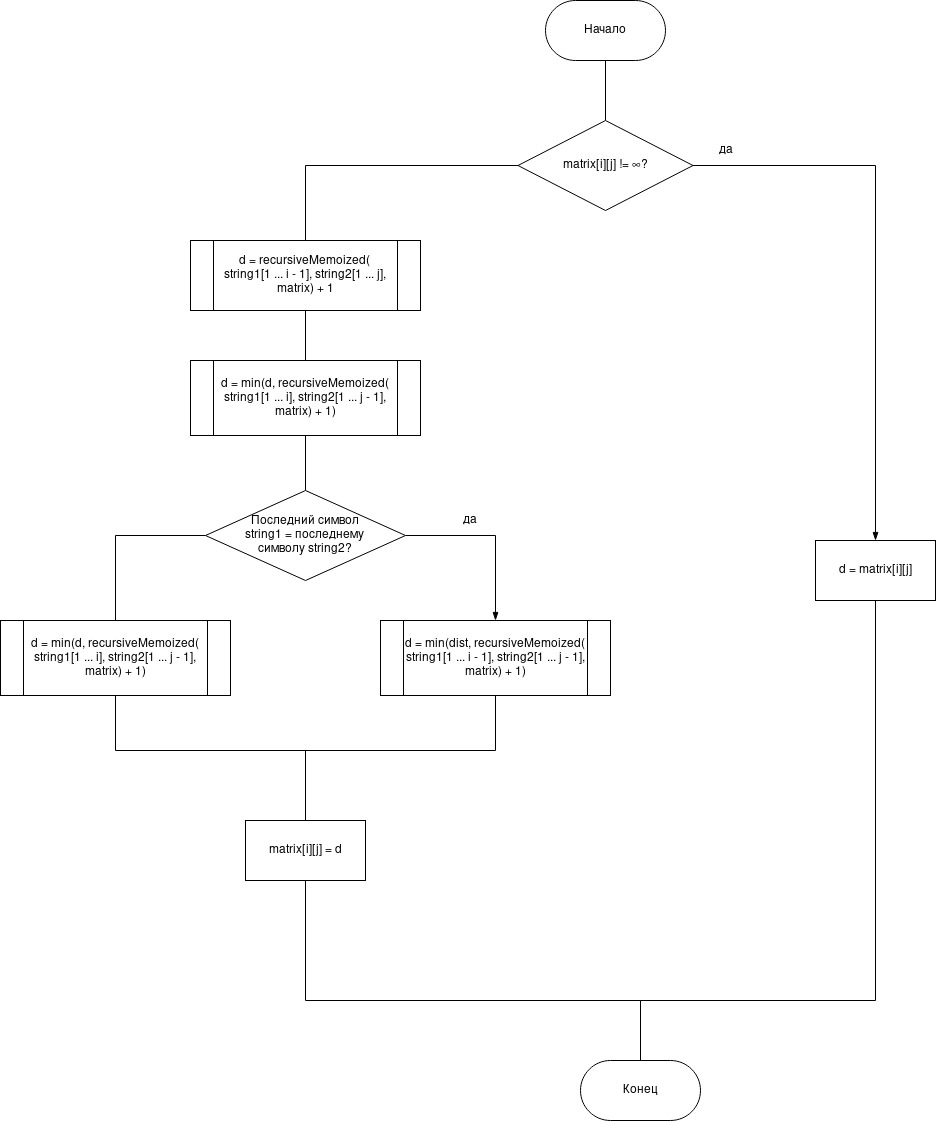
\includegraphics[scale=0.45]{mem.jpg}
	\caption{Схема рекурсивного алгоритма с мемоизацией нахождения расстояния Левенштейна}
	\label{fig:mpr}
\end{figure}

\begin{figure}[h]
	\centering
	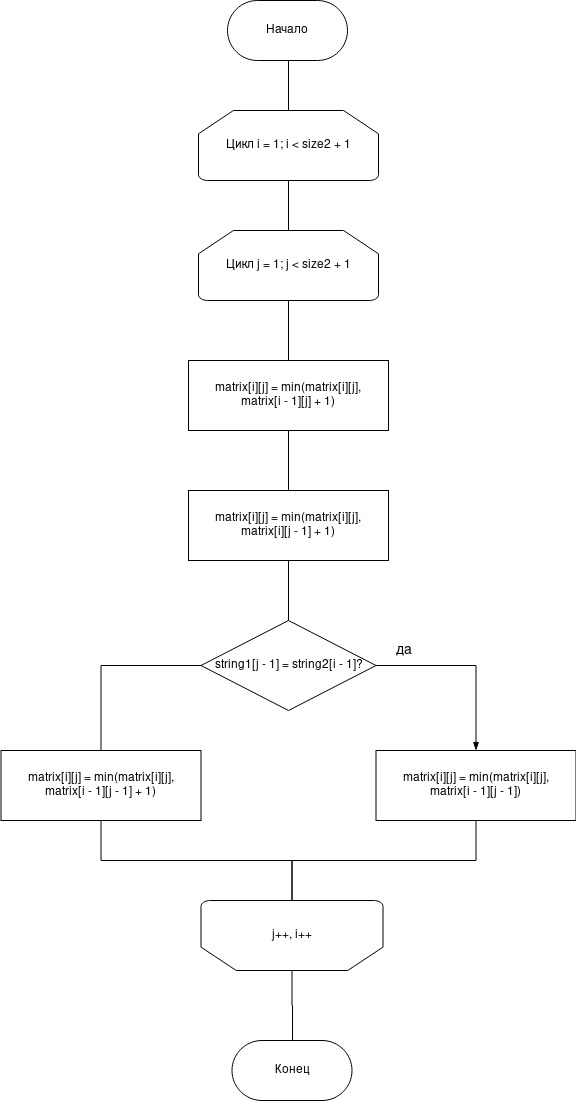
\includegraphics[scale=0.6]{iter.jpg}
	\caption{Схема итеративного алгоритма нахождения расстояния Левенштейна}
	\label{fig:mpr}
\end{figure}

\begin{figure}[h]
	\centering
	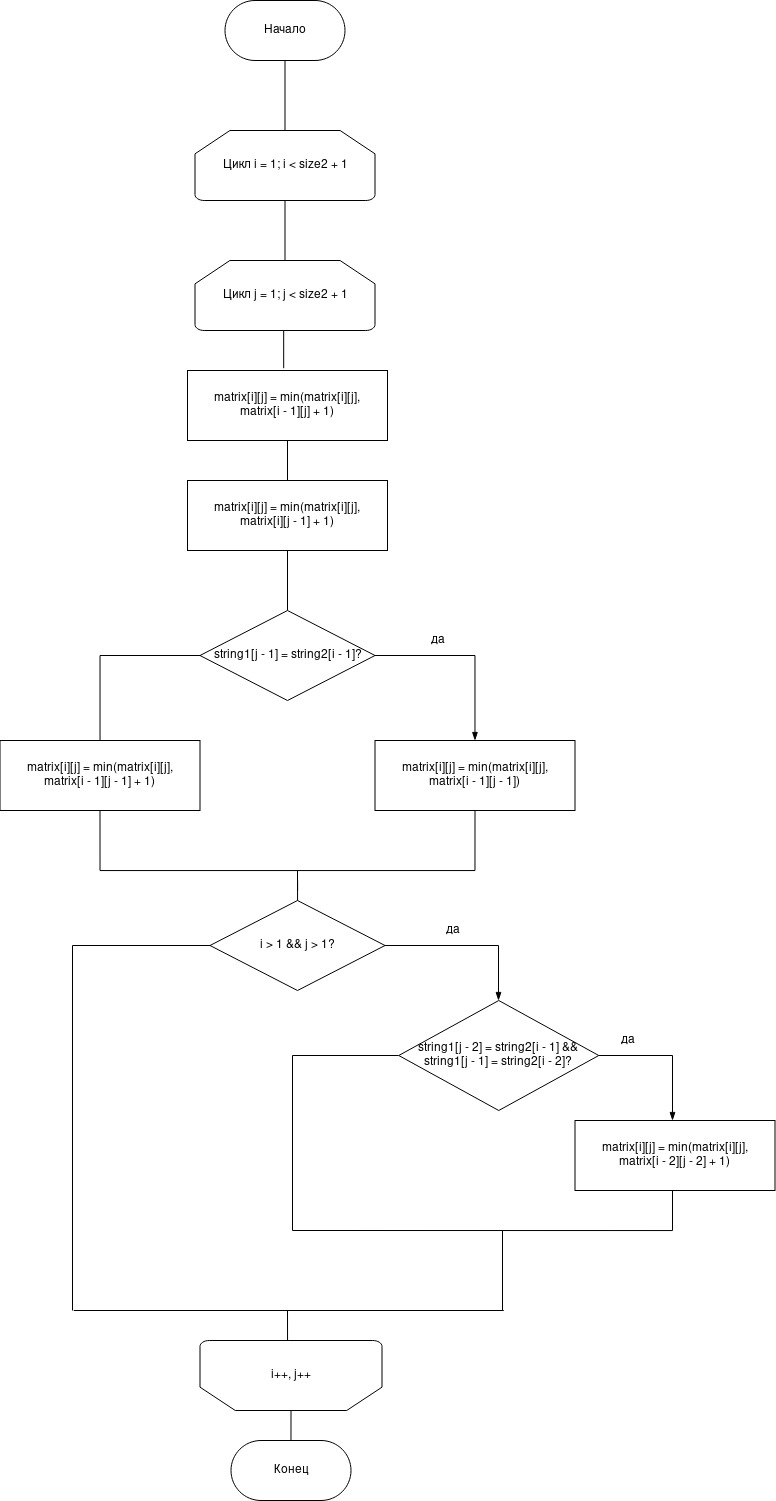
\includegraphics[scale=0.4]{iter_dl.jpg}
	\caption{Схема итеративного алгоритма нахождения расстояния Дамерау-Левенштейна}
	\label{fig:mpr}
\end{figure}

\section{Модель вычислений}

\section{Трудоёмкость алгоритмов}

\subsection{Стандартный алгоритм умножения матриц}

\subsection{Алгоритм Копперсмита — Винограда}

\subsection{Оптимизированный алгоритм Копперсмита — Винограда}

\section{Вывод}
	На основе теоретических данных, полученных из аналитического раздела, были построены схемы обоих алгоритмов умножения матриц.  Оценены их трудоёмкости в лучшем и худшем случаях.

\chapter{Технологическая часть}

В данном разделе приведены средства реализации и листинги кода.

\section{Требование к ПО}

К программе предъявляется ряд требований:

\begin{itemize}

	\item На вход ПО получает размеры 2 матриц, а также их элементы;

	\item На выходе — ПО печатает матрицу, которая является результатом умножения входных матриц.

\end{itemize}

\section{Средства реализации}
Для реализации ПО я выбрал язык программирования Haskell \cite{Haskell}. Данный выбор обусловлен моим желанием расширить свои знания в области применения данного язкыа программирования. 

\section{Реализация алгоритмов}

В листингах 3.1 - 3.4 приведена реализация алгоритмов перемножения матриц.

\begin{lstlisting}[label=some-code,caption=Функция умножения матриц обычным способом, language=Haskell]
baseMultiplication :: (Num a) => Matrix a -> Matrix a -> Matrix a
baseMultiplication m1 m2 = M.fromList (M.ncols m2) (M.nrows m1) $ V.toList $ _multp m1 m2 1
  where
    _multp m1 m2 i
    | i == M.nrows m1 + 1 = V.fromList []
    | otherwise = P.foldl (\acc j ->
      V.zipWith (+) acc $ V.zipWith (*) (V.fromList $ P.take (M.nrows m1) $ repeat (M.getElem i j m1)) (M.getRow j m2))
     (V.fromList $ P.take (M.ncols m2) $ repeat 0) [1..M.ncols m1] V.++ _multp m1 m2 (i + 1)
\end{lstlisting}

\begin{lstlisting}[label=some-code,caption=Функция умножения матриц с транспонированием,language=Haskell]
baseTMultiplication :: (Num a) => Matrix a -> Matrix a -> Matrix a
baseTMultiplication m1 m2 =  M.fromList (M.ncols m2) (M.nrows m1) $ V.toList $ _multp m1 (M.transpose m2) 1
  where
    _multp m1 m2 i
      | i == M.nrows m1 + 1 = V.fromList []
      | otherwise = P.foldl (\acc j ->
        V.snoc acc $ V.sum (V.zipWith (*) (M.getRow i m1) (M.getRow j m2))) (V.fromList []) [1..M.nrows m2]
        V.++ _multp m1 m2 (i + 1)
\end{lstlisting}

\begin{lstlisting}[label=some-code,caption=Функция умножения матриц по Винограду,language=Haskell]
winogradMultiplication :: (Num a) => Matrix a -> Matrix a -> Matrix a
winogradMultiplication m1 m2 = res
  where
    a = M.nrows m1
    b = M.ncols m1
    c = M.ncols m2

    rows = V.generate a $ \i -> precalc $ M.getRow (i + 1) m1
    cols = V.generate c $ \j -> precalc $ M.getCol (j + 1) m2

    precalc v = P.foldl (\acc i ->
    acc - V.unsafeIndex v i * V.unsafeIndex v (i + 1)) 0 [0, 2 .. V.length v - 2]
	
    res = M.matrix a c $ \(i, j) ->
      V.unsafeIndex rows (i - 1) + V.unsafeIndex cols (j - 1)
      + subcalc (M.getRow i m1) (M.getCol j m2)
      + if odd b then M.unsafeGet i b m1 * M.unsafeGet b j m2 else 0
	
    subcalc v1 v2 = P.foldl (\acc i ->
    acc + (V.unsafeIndex v1 (i + 1) + V.unsafeIndex v2 (i))
        * (V.unsafeIndex v1 (i) + V.unsafeIndex v2 (i + 1))) 0 [0, 2 .. V.length v1 - 2]
\end{lstlisting}


\begin{lstlisting}[label=some-code,caption=Функция нахождения расстояния Дамерау-Левенштейна матрично,language=Haskell]
winogradOptimizedMultiplication :: (Num a) => Matrix a -> Matrix a -> Matrix a
winogradOptimizedMultiplication m1 m2 = res
  where
    a = M.nrows m1
    b = M.ncols m1
    c = M.ncols m2
	
    m1' = V.generate a $ \i -> M.getRow (i + 1) m1
    m2' = V.generate c $ \j -> M.getCol (j + 1) m2
	
    rows = V.generate a $ \i -> precalc $ V.unsafeIndex m1' i
    cols = V.generate c $ \j -> precalc $ V.unsafeIndex m2' j
	
    precalc v = P.foldl (\acc i ->
      acc - V.unsafeIndex v i * V.unsafeIndex v (i + 1)) 0 [0, 2 ..  b - 2]
	
    res = if odd b
      then M.matrix a c $ \(i, j) ->
        let v1 = V.unsafeIndex m1' (i - 1)
            v2 = V.unsafeIndex m2' (j - 1)
        in V.unsafeIndex rows (i - 1) + V.unsafeIndex cols (j - 1) + subcalc v1 v2 + V.last v1 * V.last v2
      else M.matrix a c $ \(i, j) ->
        let v1 = V.unsafeIndex m1' (i - 1)
            v2 = V.unsafeIndex m2' (j - 1)
        in V.unsafeIndex rows (i - 1) + V.unsafeIndex cols (j - 1) + subcalc v1 v2
	
    subcalc v1 v2 = P.foldl (\acc i ->
      acc + (V.unsafeIndex v1 (i + 1) + V.unsafeIndex v2 (i))
          * (V.unsafeIndex v1 (i) + V.unsafeIndex v2 (i + 1))) 0 [0, 2 .. b - 2]
\end{lstlisting}

\section{Тестовые данные}

В таблице~\ref{tabular:test_rec} приведены тесты для функций, реализующих стандартный алгоритм умножения матриц, алгоритм Винограда и оптимизированный алгоритм Винограда. Все тесты пройдены успешно.

\begin{table}[h!]
	\begin{center}
		\begin{tabular}{c@{\hspace{7mm}}c@{\hspace{7mm}}c@{\hspace{7mm}}c@{\hspace{7mm}}c@{\hspace{7mm}}c@{\hspace{7mm}}}
			\hline
			Первая матрица & Вторая матрица & Ожидаемый результат \\ \hline
			\vspace{4mm}
			$\begin{pmatrix}
			1 & 2 & 3\\
			1 & 2 & 3\\
			1 & 2 & 3
			\end{pmatrix}$ &
			$\begin{pmatrix}
			1 & 2 & 3\\
			1 & 2 & 3\\
			1 & 2 & 3
			\end{pmatrix}$ &
			$\begin{pmatrix}
			6 & 12 & 18\\
			6 & 12 & 18\\
			6 & 12 & 18
			\end{pmatrix}$ \\
			\vspace{2mm}
			\vspace{2mm}
			$\begin{pmatrix}
			1 & 2 & 2\\
			1 & 2 & 2
			\end{pmatrix}$ &
			$\begin{pmatrix}
			1 & 2\\
			1 & 2\\
			1 & 2
			\end{pmatrix}$ &
			$\begin{pmatrix}
			5 & 10\\
			5 & 10
			\end{pmatrix}$ \\
			\vspace{2mm}
			\vspace{2mm}
			$\begin{pmatrix}
			2
			\end{pmatrix}$ &
			$\begin{pmatrix}
			2
			\end{pmatrix}$ &
			$\begin{pmatrix}
			4
			\end{pmatrix}$ \\
			\vspace{2mm}
			\vspace{2mm}
			$\begin{pmatrix}
			1 & -2 & 3\\
			1 & 2 & 3\\
			1 & 2 & 3
			\end{pmatrix}$ &
			$\begin{pmatrix}
			-1 & 2 & 3\\
			1 & 2 & 3\\
			1 & 2 & 3
			\end{pmatrix}$ &
			$\begin{pmatrix}
			0 & 4 & 6\\
			4 & 12 & 18\\
			4 & 12 & 18
			\end{pmatrix}$\\
			\vspace{2mm}
			\vspace{2mm}
		\end{tabular}
	\end{center}
	\caption{\label{tabular:test_rec} Тестирование функций}
\end{table}

\section{Вывод}

В данном разделе были разработаны исходные коды четырёх алгоритмов перемножения матриц: обычный алгоритм, алгоритм с транспонированием, алгоритм Копперсмита — Винограда, оптимизированный алгоритм Копперсмита — Винограда.

\chapter{Исследовательская часть}

\section{Технические характеристики}

Ниже приведены технические характеристики устройства, на котором было проведено тестирование ПО:

\begin{itemize}
	\item Операционная система: Debian \cite{debian} Linux \cite{linux} 11 <<bullseye>> 64-bit.
	\item Оперативная память: 12 GB.
	\item Процессор: Intel(R) Core(TM) i5-3550 CPU @ 3.30GHz
\cite{i5}.

\end{itemize}

\section{Время выполнения алгоритмов}
Время выполнения алгоритм замерялось с помощью применения технологии профайлинга \cite{profiling}. Данный инстрмуент даёт детальное описание количества вызовов и количества времени CPU, занятого каждой функцией. \newline

В таблицах 4.1 и 4.2 представлены замеры времени работы для каждого из алгоритмов на чётных размерах матриц.

\begin{table} [h!]
	\caption{Таблица времени выполнения алгоритмов при чётных размерах (в секундах)}
	\begin{center}
		\begin{tabular}{|c c c c c|} 
		 	\hline
			Размер матрицы & С & ТС & КВ & ОКВ \\  
		 	\hline
		 	100 & 0.482 & 0.120 & 0.169 & 0.158 \\
		 	\hline
		 	200 & X & X & X & 1.253 \\
		 	\hline
			300 & X & X & X & 4.063 \\
			\hline
			400 & X & X & X & 9.909 \\
			\hline
			500 & X & X & X & 19.357 \\
			\hline
			600 & X & X & X & 33.265 \\
			\hline
		\end{tabular}
	\end{center}
\end{table}

\begin{table} [h!]
	\caption{Таблица времени выполнения алгоритмов при нечётных размерах (в наносекундах)}
	\begin{center}
		\begin{tabular}{|c c c c c|} 
			\hline
			Размер матрицы & С & ТС & КВ & ОКВ \\  
			\hline
			10 & 30500400 & 1300 & 650 & 680\\
			\hline
			20 & NaN & 5100 & 2300 & 2500 \\
			\hline
			30 & NaN & 11000 & 4800 & 5200 \\
			\hline
			50 & NaN & 30000 & 12500 & 13500 \\
			\hline
			100 & NaN & 115000 & 48000 & 55000\\
			\hline
			200 & NaN & 530000 & 249000 & 528000 \\
			\hline
		\end{tabular}
	\end{center}
\end{table}




\section{Вывод}

Тут какой то вывод..

\chapter*{Заключение}
\addcontentsline{toc}{chapter}{Заключение}

В рамках данной лабораторной работы:

\begin{enumerate}

	\item Были изучены и реализованы 3 алгоритма перемножения матриц: обычный, Копперсмита -- Винограда, оптимизированный Копперсмита -- Винограда;

	\item Был произведён анализ трудоёмкости алгоритмов на основе теоретических расчётов и выбранной модели вычислений;

	\item Был сделан сравнительный анализ алгоритмов на основе экспериментальных данных;

\end{enumerate}


%На основании анализа трудоёмкости алгоритмов в выбранной модели вычислений было показано, что улучшенный алгоритм Винограда имеет меньшую сложность, нежели простой алгоритм перемножения матриц, что при размерах матриц $800 \times 800$ дало практический выигрыш во времени в 10\%.

\addcontentsline{toc}{chapter}{Литература}

\bibliographystyle{utf8gost705u}  % стилевой файл для оформления по ГОСТу

\bibliography{51-biblio}          % имя библиографической базы (bib-файла)


\end{document}
